\documentclass[a4paper, 10pt]{article}
\usepackage{../../CEDT-Homework-style}

\usepackage{amsmath}
\allowdisplaybreaks

\setlength{\headheight}{14.49998pt}

\begin{document}
\subject[2110203 - Computer Engineering Mathematics II]
\hwtitle{Signal 3}{}{Week 3}{6733172621 Patthadon Phengpinij}{ChatGPT (for\,\LaTeX\,styling and grammar checking)}


% ================================================================================ %
\section{Fourier Series}
% ================================================================================ %



% ================================================================================ %
%                                    Problem 01                                    %
% ================================================================================ %
\begin{problem}
Find the Fourier series of the following periodic function:

\begin{center}
    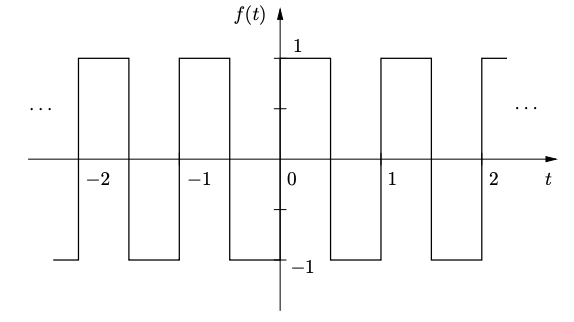
\includegraphics[width=0.6\textwidth]{images/problem_1_reference.png}
\end{center}
\end{problem}

\begin{solution}
The signal in the image is a periodic signum function with period \( T = 1 \) and amplitude \( A = 1 \). The function can be defined as:
\[ x(t) = 
\begin{cases}
1, & 0 \leq t < 0.5 \\
-1, & 0.5 \leq t < 1
\end{cases} \]
To find the Fourier series coefficients, we use the formulas for \( a_0 \), \( a_n \), and \( b_n \):
\[ a_0 = \frac{1}{T} \int_{0}^{T} x(t) \, dt \]
\[ a_n = \frac{2}{T} \int_{0}^{T} x(t) \cos\paren{ \frac{2\pi n t}{T} } dt \]
\[ b_n = \frac{2}{T} \int_{0}^{T} x(t) \sin\paren{ \frac{2\pi n t}{T} } dt \]

Calculating \( a_0 \):
\begin{align*}
    a_0 &= \frac{1}{1} \int_{0}^{1} x(t) \, dt \\
    &= \frac{1}{1} \paren{ \int_{0}^{0.5} 1 \, dt + \int_{0.5}^{1} -1 \, dt } \\
    &= \paren{ 0.5 - 0.5 } \\
    a_0 &= 0
\end{align*}

\newpage

Calculating \( a_n \):
\begin{align*}
    a_n &= \frac{2}{1} \int_{0}^{1} x(t) \cos(2\pi n t) \, dt \\
    &= 2 \paren{ \int_{0}^{0.5} (1) \cdot \cos(2\pi n t) \, dt + \int_{0.5}^{1} (-1) \cdot \cos(2\pi n t) \, dt } \\
    &= 2 \paren{ \sqbracket{ \frac{\sin(2\pi n t)}{2\pi n} }_{0}^{0.5} - \sqbracket{ \frac{\sin(2\pi n t)}{2\pi n} }_{0.5}^{1} } \\
    &= \frac{2}{2\pi n} \sqbracket{ \paren{ \sin(\pi n) - \sin(0) } - \paren{ \sin(2\pi n) - \sin(\pi n) } } \\
    &= \frac{1}{\pi n} \sqbracket{ 0 } \\
    a_n &= 0
\end{align*}

Calculating \( b_n \):
\begin{align*}
    b_n &= \frac{2}{1} \int_{0}^{1} x(t) \sin(2\pi n t) \, dt \\
    &= 2 \paren{ \int_{0}^{0.5} (1) \cdot \sin(2\pi n t) \, dt + \int_{0.5}^{1} (-1) \cdot \sin(2\pi n t) \, dt } \\
    &= 2 \paren{ \sqbracket{ -\frac{\cos(2\pi n t)}{2\pi n} }_{0}^{0.5} - \sqbracket{ -\frac{\cos(2\pi n t)}{2\pi n} }_{0.5}^{1} } \\
    &= \frac{2}{2\pi n} \sqbracket{ \paren{ -\cos(\pi n) + \cos(0) } - \paren{ -\cos(2\pi n) + \cos(\pi n) } } \\
    &= \frac{1}{\pi n} \sqbracket{ 2\paren{ 1 - \cos(\pi n) } } \\
    &= \frac{2}{\pi n} \paren{ 1 - (-1)^n } \\
    b_n &= \begin{cases} \frac{4}{\pi n}, & n \text{ odd} \\ 0, & n \text{ even} \end{cases}
\end{align*}

Because, in term of \( a_0 \), \( a_n \), \( b_n \), we have:
\[ x(t) = a_0 + \sum_{n=1}^{\infty} \paren{ a_n \cos(2\pi n t) + b_n \sin(2\pi n t) } \]
and we found that \( a_0 = 0 \), \( a_n = 0 \), and \( b_n = \frac{4}{\pi n} \) for odd \( n \) and \( 0 \) for even \( n \).

Therefore, the Fourier series representation of the signal is:
\[ x(t) = \sum_{n=1, n \text{ odd}}^{\infty} \frac{4}{\pi n} \sin(2\pi n t) \]
\end{solution}
% ================================================================================ %

\newpage

% ================================================================================ %
%                                    Problem 02                                    %
% ================================================================================ %
\begin{problem}
Find the Fourier Series (FS) of the periodic function \( x(t) \) which are provided as follows.
\end{problem}


% === Problem 2.1. === %
\begin{subproblems}[start=1]
    \item \( x(t) = \frac{\pi t^3}{2};\; -1 < t < 1 \)
\end{subproblems}

\begin{solution}

\end{solution}
% ==================== %

\newpage 

% === Problem 2.2. === %
\begin{tosubmit}
\begin{subproblems}[start=2]
    \item \( x(t) = \pi - t;\; -\pi \leq t \leq \pi \)
\end{subproblems}

\par\noindent\submitsolution

\end{tosubmit}
% ==================== %

\newpage

% === Problem 2.3. === %
\begin{tosubmit}
\begin{subproblems}[start=3]
    \item \( x(t) = t^2 + \sin^3(\pi t);\; -1 \leq t \leq 1 \)
\end{subproblems}

\par\noindent\submitsolution

\end{tosubmit}
% ==================== %
% ================================================================================ %


\end{document}